\documentclass[tikz,crop]{standalone}

\usepackage{tikz}
\usepackage{xcolor}
\usepackage{pgfplots}
\usepackage{siunitx}
\usepackage{fontspec}
\setmainfont{Source Serif 4}[
    Renderer = OpenType,
    SizeFeatures    = {%
        {Size={-9},Font=* Caption},
        {Size={9-13},Font=*},
        {Size={14-24},Font=* Subhead},
        {Size={24-},Font=* Display}
    },
    ItalicFeatures = {%
    SizeFeatures    = {%
            {Size={-9},Font=* Caption Italic},
            {Size={9-13},Font=* Italic},
            {Size={14-24},Font=* Subhead Italic},
            {Size={24-},Font=* Display Italic}
    },
    },
    BoldFeatures = {%
    SizeFeatures    = {%
            {Size={-9},Font=* Caption Semibold},
            {Size={9-13},Font=* Semibold},
            {Size={14-24},Font=* Subhead Semibold},
            {Size={24-},Font=* Display Semibold}
    },
    },
    BoldItalicFeatures = {%
    SizeFeatures    = {%
            {Size={-9},Font=* Caption Semibold Italic},
            {Size={9-13},Font=* Semibold Italic},
            {Size={14-24},Font=* Subhead Semibold Italic},
            {Size={24-},Font=* Display Semibold Italic}
    },
    },
    Numbers         = OldStyle,
]

\pgfplotsset{compat=1.18}
\usepgfplotslibrary{statistics}

\usetikzlibrary{shapes,arrows,positioning,backgrounds,calc,intersections,calc,svg.path,fit}

\definecolor{ugent-re}{RGB}{220, 78, 40}        % vermilion			/ vermiljoen
\definecolor{ugent-we}{RGB}{45, 140, 168}       % no match
\definecolor{ugent-ge}{RGB}{232, 94, 113}       % rose				/ bleekrood
\definecolor{ugent-ea}{RGB}{111, 113, 185}      % distant blue		/ verblauw
\definecolor{ugent-pp}{RGB}{251, 126, 58}       % deep orange		/ dieporanje
\definecolor{ugent-ps}{RGB}{113, 168, 96}       % yellow green		/ geelgroen

\usepackage{xparse}

\begin{document}

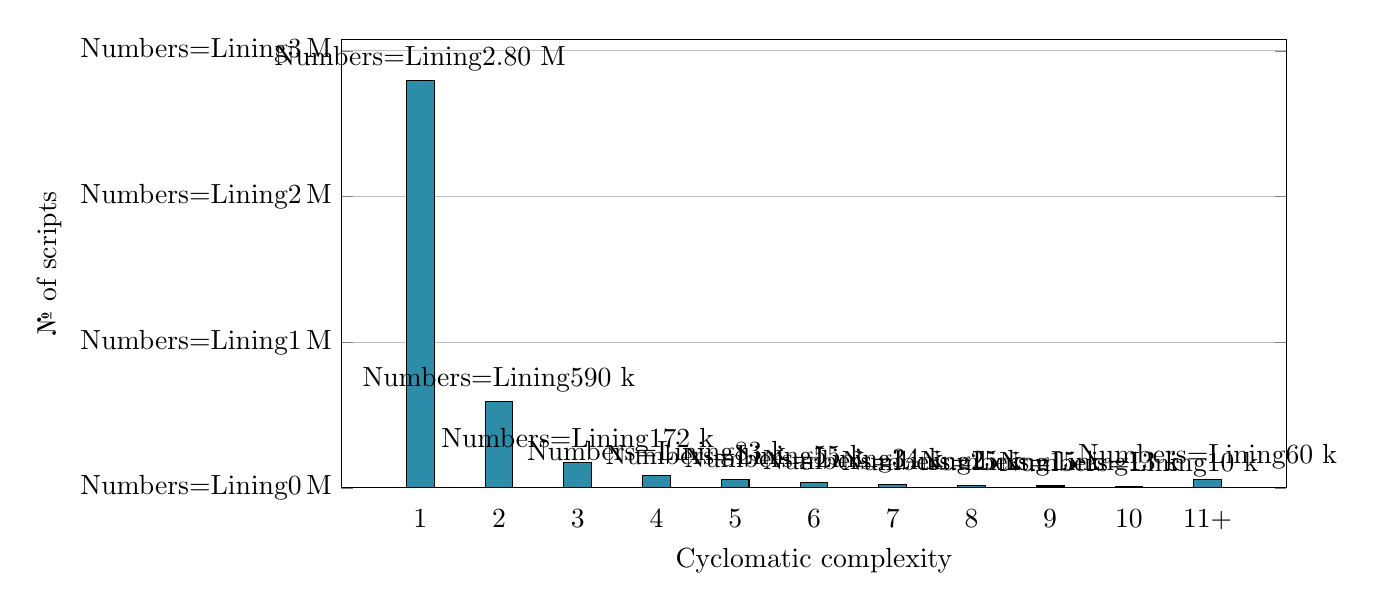
\begin{tikzpicture}
    \begin{axis}[
        ybar,
        ymin=0,
        x=1cm,
        ylabel style={align=center},
        ylabel={№ of scripts},
        xlabel={Cyclomatic complexity},
        nodes near coords={%
            \addfontfeature{Numbers={Lining}}%
            \pgfmathfloattofixed{\pgfplotspointmeta}%
            \edef\val{\pgfmathresult}%
            \pgfkeys{/pgf/fpu}%
            \pgfmathsetmacro\ccexponente{ifthenelse(\val<1000000,3,6))}%
            \pgfmathfloattoint{\ccexponente}%
            \edef\ccexponent{\pgfmathresult}%
            \pgfkeys{/pgf/fpu=false}%
            \pgfmathsetmacro\ccsuffix{ifthenelse(\ccexponent==3,"k","M"))}%
            \pgfmathsetmacro\ccround{ifthenelse(\ccexponent==3,0,2))}%
            \num[round-mode=places,round-precision=\ccround,fixed-exponent=\ccexponent,exponent-mode=fixed,drop-exponent=true]{\val}\ \ccsuffix
        },
        xtick style={draw=none},
        xtick=data,
        ymajorgrids,
        yminorgrids,
        xticklabels={1,2,...,10,11+},
        scaled y ticks=false,
        yticklabel={\addfontfeature{Numbers={Lining}}\qty[round-mode=places, round-precision=0,fixed-exponent=6,exponent-mode=fixed,drop-exponent=true]{\tick}{\mega{}}},
        bar shift=0pt
    ]
        \addplot[style={fill=ugent-we}] coordinates {
            (1,2797997)
            (2,589626)
            (3,172432)
            (4,82891)
            (5,55188)
            (6,34297)
            (7,24828)
            (8,14677)
            (9,12766)
            (10,10219)
            (11,59947)
        };
    \end{axis}
\end{tikzpicture}

\end{document}
